% Provenance (never printed): old seconde/premiere S material on the
% atmosphere (storms, cyclones, the energy of the water cycle) and the
% natural-hazard themes of SVT; see sources/book2/PROVENANCE.md. Tracks,
% genesis statistics and the pressure--wind relation are computed in
% figdata/grade-10/cyclones.py from IBTrACS v04r01; the surge, thunder and
% energy numbers in the same script.
\chapter{Trovoadas e ciclones tropicais}\label{ch:g10:storms-and-cyclones}

Uma tarde quente de verão termina em temporal. O céu escurece, uma rajada
de vento frio varre a rua, um clarão ilumina as nuvens --- e você começa a
contar: um, dois, três, \ldots{} nove segundos depois, o trovão ribomba. A
tempestade está a uns três quilômetros. Em uma hora ela terá passado, e o ar
estará fresco e limpo. Sobre os oceanos tropicais quentes, os mesmos
ingredientes --- ar quente e úmido que sobe e se condensa --- podem se
organizar em tempestades de um tamanho completamente diferente: os \omterm{def:g10:storms-and-cyclones:tropical-cyclone}{ciclones
tropicais}, com centenas de quilômetros de diâmetro, que duram dias e trazem
ventos fortes o bastante para derrubar florestas e uma subida do mar que
inunda costas inteiras. Este capítulo trata das \omterm{def:g10:storms-and-cyclones:thunderstorm}{trovoadas}, dos \omterm{def:g10:storms-and-cyclones:tornado}{tornados} e
dos \omterm{def:g10:storms-and-cyclones:tropical-cyclone}{ciclones tropicais}, e de onde vem a sua energia.

\begin{safety}
Se você consegue ouvir o trovão, o \omterm{def:g10:storms-and-cyclones:lightning}{raio} pode atingi-lo. Entre num prédio ou
num carro fechado e fique ali até bem depois do último trovão. Nunca se
abrigue sob uma árvore isolada, e fique longe do alto dos morros, dos campos
abertos e da água.
\end{safety}

\begin{recall}
As massas de ar, as frentes, as depressões (zonas de baixa pressão) e os
anticiclones são desenhados nas cartas do tempo com isóbaras, linhas de
mesma pressão (Livro 1, 8º ano). Uma ameaça natural é um fenômeno natural
que pode causar danos às pessoas e ao que elas constroem (Livro 1, 5º ano).
O som se propaga no ar a cerca de \qty{340}{m/s}, e a luz quase
instantaneamente (os livros de física). O ar quente e úmido que sobe se
resfria, se condensa em nuvem no seu \omterm{def:g10:why-clouds-form:condensation-level}{nível de condensação} e libera \omterm{def:g10:earth-energy-budget:latent-heat}{calor
latente}; o ar saturado é muitas vezes instável
(\cref{ch:g10:why-clouds-form}).
\end{recall}

\section{As trovoadas}

\begin{definition}[Trovoada]\label{def:g10:storms-and-cyclones:thunderstorm}
Uma \emph{trovoada}\index{trovoada} é uma tempestade produzida por uma nuvem
cumulonimbo, com \omterm{def:g10:storms-and-cyclones:lightning}{raios} e trovões, em geral com aguaceiros fortes e rajadas
de vento, às vezes com granizo.
\end{definition}

Uma \omterm{def:g10:storms-and-cyclones:thunderstorm}{trovoada} nasce de um \omterm{def:g10:why-clouds-form:stability}{ar instável} e úmido. Na primeira fase, um cúmulo
cresce para cima, alimentado por uma forte corrente ascendente; a
condensação libera \omterm{def:g10:earth-energy-budget:latent-heat}{calor latente} e mantém o ar que sobe mais quente que o
ar em volta. Na fase madura, a nuvem chega ao \omterm{def:g10:why-clouds-form:stability}{ar estável} lá no alto e se
espalha numa bigorna; gotas e pedras de granizo ficam grandes o bastante
para cair, e a chuva que cai arrasta consigo o ar frio para baixo: uma
corrente descendente que se espalha junto ao chão numa frente de rajada
fria. Na última fase, a corrente descendente toma conta da nuvem inteira,
cortando o fornecimento de ar quente e úmido, e a tempestade se esgota em
chuva.

\begin{omfigure}
\begin{tikzpicture}[font=\footnotesize, >={Stealth[length=2mm]}]
  \foreach \dx/\title in {0/{1. em crescimento}, 4.6/{2. madura}, 9.2/{3. em dissipação}}
    \node[anchor=north] at (\dx+1.6,-0.15) {\title};
  \draw[thick, black!60] (-0.3,0) -- (12.9,0);
  % stage 1: a tall cumulus
  \pic[scale=1.4, transform shape] at (1.6,1.2) {puffycloud};
  \pic[scale=1.1, transform shape] at (1.6,2.0) {puffycloud};
  \foreach \x in {1.2,1.6,2.0} \draw[->, thick, omThm!80!black] (\x,0.2) -- (\x,2.6);
  % stage 2: cumulonimbus with anvil
  \fill[black!8, draw=black!50] (5.0,1.0) -- (4.9,4.0) -- (4.2,4.4) -- (8.0,4.6) -- (7.4,4.0) -- (7.2,1.0) -- cycle;
  \draw[->, thick, omThm!80!black] (5.5,0.2) -- (5.5,4.2);
  \draw[->, thick, omThm!80!black] (5.9,0.2) -- (5.9,4.2);
  \draw[->, thick, omDef!80!black] (6.7,3.4) -- (6.7,0.3) -- (7.6,0.3);
  \foreach \x in {6.4,6.85,7.05} \draw[omDef!50] (\x,0.95) -- (\x-0.1,0.1);
  \node[anchor=west, align=left] at (8.0,4.6) {bigorna};
  \node[anchor=west, align=left, omDef!80!black] at (7.65,0.45) {frente de rajada};
  % stage 3: dissipating
  \fill[black!8, draw=black!50] (9.7,1.2) -- (9.6,3.6) -- (9.0,4.0) -- (12.6,4.1) -- (12.0,3.6) -- (11.8,1.2) -- cycle;
  \foreach \x in {10.3,10.9,11.5} \draw[->, thick, omDef!80!black] (\x,3.2) -- (\x,0.3);
  \foreach \x in {10.6,11.2} \draw[omDef!50] (\x,1.15) -- (\x-0.1,0.1);
  % legend
  \draw[->, thick, omThm!80!black] (0,5.0) -- (0,5.5); \node[anchor=west] at (0.1,5.25) {ar quente que sobe};
  \draw[->, thick, omDef!80!black] (3.2,5.5) -- (3.2,5.0); \node[anchor=west] at (3.3,5.25) {ar frio que desce};
\end{tikzpicture}

{\small As três fases de uma \omterm{def:g10:storms-and-cyclones:thunderstorm}{trovoada} (esquema, fora de escala): um cúmulo
em crescimento alimentado por correntes ascendentes; o cumulonimbo maduro,
com a sua bigorna, a sua corrente ascendente e uma corrente descendente
arrastada pela chuva; a tempestade em dissipação, só corrente descendente.}
\end{omfigure}

Dentro da nuvem, as colisões entre partículas de gelo levadas para cima e
para baixo pelo ar separam cargas elétricas: a nuvem fica carregada, em
geral negativamente embaixo e positivamente em cima, e o chão sob ela ganha
uma carga própria.

\begin{definition}[Raio]\label{def:g10:storms-and-cyclones:lightning}
O \emph{raio}\index{raio} é uma faísca elétrica gigante que descarrega as
regiões carregadas de uma tempestade, dentro da nuvem, entre nuvens ou entre
a nuvem e o chão. Ele aquece um canal estreito de ar tão de repente que o ar
se expande num choque: o som dessa expansão é o \emph{trovão}.
\end{definition}

\begin{omfigure}
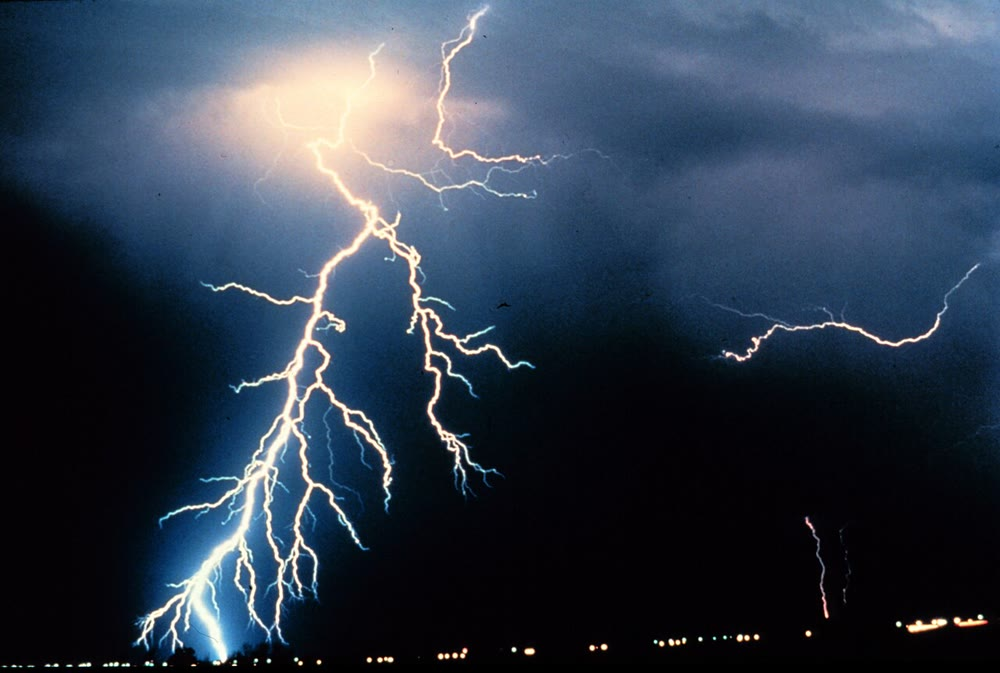
\includegraphics[width=0.62\linewidth]{images/book2/g10-noaa-lightning.jpg}

{\small \omterm{def:g10:storms-and-cyclones:lightning}{Raios}, entre nuvens e da nuvem ao chão, durante uma \omterm{def:g10:storms-and-cyclones:thunderstorm}{trovoada}
noturna. Fotografia: C.~Clark, NOAA National Severe Storms Laboratory
(domínio público).}
\end{omfigure}

Os satélites que contam os clarões de luz sobre o planeta inteiro encontram
cerca de 1.4 bilhão de \omterm{def:g10:storms-and-cyclones:lightning}{raios} por ano, ou 44 a cada segundo.
% ledger: christian:flash-rate

\begin{method}[A distância de uma tempestade, do clarão ao trovão]\label{met:g10:storms-and-cyclones:distance}
\begin{enumerate}
  \item A luz do clarão chega praticamente na hora; o trovão viaja à
        velocidade do som, cerca de \qty{343}{m/s} a
        \qty{20}{\degreeCelsius}.
  \item Conte os segundos $t$ entre o clarão e o trovão.
  \item A distância é de $343\,t$ metros: cerca de \qty{1}{km} a cada três
        segundos.
\end{enumerate}
\end{method}
% ledger: const:R, earth:Mmol (speed of sound computed in figdata/grade-10/cyclones.py)

\section{Os tornados}

\begin{definition}[Tornado]\label{def:g10:storms-and-cyclones:tornado}
Um \emph{tornado}\index{tornado} é uma coluna de ar em rotação violenta, em
contato com o chão, pendurada na base de um cumulonimbo.
\end{definition}

Os \omterm{def:g10:storms-and-cyclones:tornado}{tornados} mais fortes vêm das \emph{supercélulas}, \omterm{def:g10:storms-and-cyclones:thunderstorm}{trovoadas} cuja corrente
ascendente gira como um todo. Um \omterm{def:g10:storms-and-cyclones:tornado}{tornado} é pequeno e breve: tipicamente
algumas centenas de metros de diâmetro, durando minutos, com uma trajetória
média de cerca de \qty{5.6}{km}. Mas os seus ventos são os mais fortes da
superfície da Terra: um radar móvel mediu cerca de \qty{135}{m/s} (uns
\qty{480}{km/h}) acima do chão num \omterm{def:g10:storms-and-cyclones:tornado}{tornado} em Oklahoma, em maio de 1999. Os
Estados Unidos têm mais \omterm{def:g10:storms-and-cyclones:tornado}{tornados} que qualquer outro país, cerca de 1200 por
ano; entre as outras regiões onde eles são frequentes estão as pradarias
canadenses, Bangladesh, o norte da Argentina e o sul do Brasil, e a
Grã-Bretanha.
% ledger: spc:tornado

\begin{omfigure}
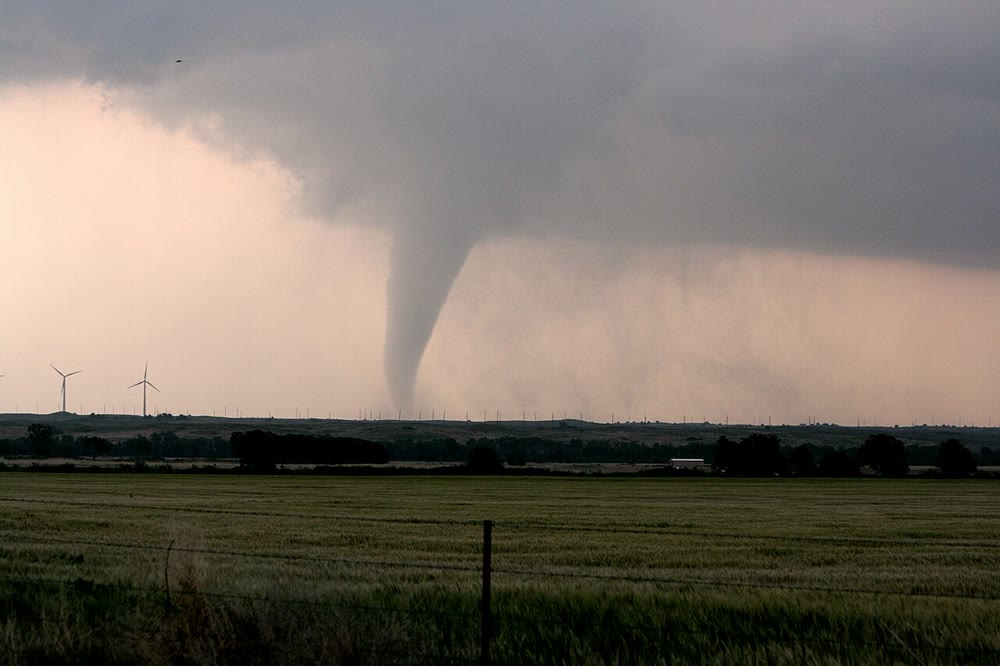
\includegraphics[width=0.62\linewidth]{images/book2/g10-noaa-tornado-kansas.jpg}

{\small Um \omterm{def:g10:storms-and-cyclones:tornado}{tornado} sobre as planícies do Kansas, em maio de 2008: o funil
pende da base da nuvem de tempestade. Fotografia: Sean Waugh, NOAA National
Severe Storms Laboratory (domínio público).}
\end{omfigure}

\section{Os ciclones tropicais}

\begin{definition}[Ciclone tropical; olho; parede do olho]\label{def:g10:storms-and-cyclones:tropical-cyclone}
Um \emph{ciclone tropical}\index{ciclone tropical} é uma tempestade, com
centenas de quilômetros de diâmetro, que se forma sobre um mar tropical
quente em torno de um centro de baixa pressão, com ventos que espiralam em
direção ao centro e faixas de \omterm{def:g10:storms-and-cyclones:thunderstorm}{trovoadas}. Quando os seus ventos sustentados
chegam a \num{64}~nós, cerca de \qty{119}{km/h}, ele é chamado de furacão
no Atlântico e no Pacífico leste, de tufão no Pacífico oeste, e
simplesmente de ciclone no oceano Índico e no Pacífico Sul. O seu centro
calmo e quase sem nuvens é o \emph{olho}\index{olho (de um ciclone)}; o
anel de \omterm{def:g10:storms-and-cyclones:thunderstorm}{trovoadas} altíssimas em volta dele, onde os ventos são mais fortes,
é a \emph{parede do olho}\index{parede do olho}.
\end{definition}
% ledger: nhc:sshws

\begin{omfigure}
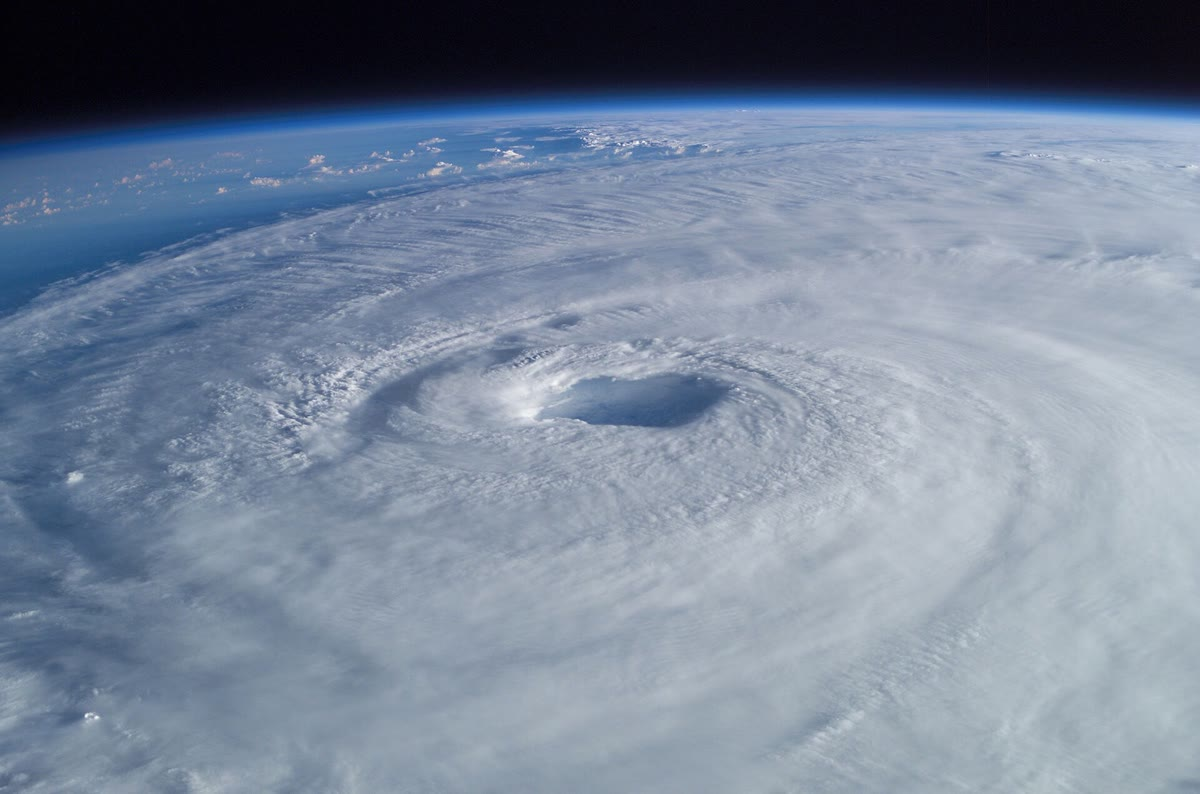
\includegraphics[width=0.78\linewidth]{images/book2/g10-nasa-hurricane-isabel.jpg}

{\small O furacão Isabel, em 15 de setembro de 2003, fotografado por um
astronauta da Estação Espacial Internacional: o \omterm{def:g10:storms-and-cyclones:tropical-cyclone}{olho}, a \omterm{def:g10:storms-and-cyclones:tropical-cyclone}{parede do olho} e a
espiral de nuvens em volta deles. Imagem: Mike Trenchard, Earth Sciences and
Image Analysis Laboratory, NASA Johnson Space Center (domínio público).}
\end{omfigure}

Perto da superfície do mar, o ar úmido flui em direção à baixa pressão do
centro. A rotação da Terra desvia o ar em movimento para a direita no
hemisfério norte: em vez de ir direto para o centro, o ar gira em torno
dele, no sentido anti-horário visto de cima (no sentido horário no
hemisfério sul). Perto do centro, ele sobe na \omterm{def:g10:storms-and-cyclones:tropical-cyclone}{parede do olho}, se condensa e
escoa pelo topo da tempestade. No \omterm{def:g10:storms-and-cyclones:tropical-cyclone}{olho}, um pouco de ar desce, se aquece e
se seca: o céu se abre.

\begin{omfigure}
\begin{tikzpicture}[font=\footnotesize, >={Stealth[length=2mm]}]
  \fill[omDef!25] (-6,-0.4) rectangle (6,0);
  \node[anchor=north, omDef!80!black] at (0,-0.05) {mar quente};
  % rain bands
  \foreach \x/\h in {-5.0/1.6, -3.9/2.2, 3.9/2.2, 5.0/1.6}
    \fill[black!10, draw=black!45] (\x-0.35,0.4) -- (\x-0.3,\h) .. controls (\x-0.15,\h+0.35) and (\x+0.15,\h+0.35) .. (\x+0.3,\h) -- (\x+0.35,0.4) -- cycle;
  % eyewall towers and outflow canopy
  \fill[black!14, draw=black!50] (-2.4,0.4) -- (-2.5,4.0) -- (-5.8,4.3) -- (-5.6,4.7) -- (-1.0,4.9) -- (-0.75,4.0) -- (-0.8,0.4) -- cycle;
  \fill[black!14, draw=black!50] (2.4,0.4) -- (2.5,4.0) -- (5.8,4.3) -- (5.6,4.7) -- (1.0,4.9) -- (0.75,4.0) -- (0.8,0.4) -- cycle;
  % inflow, rise, outflow, eye subsidence
  \draw[->, thick, omThm!80!black] (-5.8,0.2) -- (-1.3,0.2) -- (-1.3,4.3) -- (-4.2,4.45);
  \draw[->, thick, omThm!80!black] (5.8,0.2) -- (1.3,0.2) -- (1.3,4.3) -- (4.2,4.45);
  \draw[->, thick, omDef!80!black] (0,4.3) -- (0,1.0);
  \node[anchor=south, align=center] at (0,5.0) {olho: ar seco\\que desce};
  \node[anchor=south east, align=right] at (-2.6,4.95) {parede do olho};
  \node[anchor=west, align=left] at (-5.95,2.9) {faixas\\de chuva};
  \node[anchor=north, align=center] at (-3.6,0.15) {entrada de ar úmido};
  \node[anchor=south east, align=right] at (5.8,4.95) {saída em altitude};
  % plan view
  \begin{scope}[shift={(8.4,2.3)}]
    \draw[black!40] (0,0) circle (1.7);
    \foreach \a in {0,90,180,270}
      \draw[->, thick, omThm!80!black, domain=0:200, samples=30, variable=\t]
        plot ({(1.6-0.0045*\t)*cos(\a+\t)}, {(1.6-0.0045*\t)*sin(\a+\t)});
    \fill[white, draw=black!50] (0,0) circle (0.22);
    \node[anchor=north, align=center] at (0,-1.8) {visto de cima\\(hemisfério norte)};
  \end{scope}
\end{tikzpicture}

{\small Um \omterm{def:g10:storms-and-cyclones:tropical-cyclone}{ciclone tropical} em corte (esquema, altura muito exagerada): o ar
úmido entra sobre o mar quente, sobe na \omterm{def:g10:storms-and-cyclones:tropical-cyclone}{parede do olho} e nas faixas de
chuva e sai pelo topo; um pouco de ar desce no \omterm{def:g10:storms-and-cyclones:tropical-cyclone}{olho}. À direita: visto de
cima, no hemisfério norte, o ar que entra gira no sentido anti-horário em
torno do centro.}
\end{omfigure}

Os \omterm{def:g10:storms-and-cyclones:tropical-cyclone}{ciclones tropicais} precisam de um oceano quente: água de pelo menos cerca
de \qty{27}{\degreeCelsius} na superfície, quente até uma profundidade de
uns \qty{46}{m}. Eles não se formam no próprio equador, onde a rotação da
Terra não dá nenhum giro ao ar que entra: uma tempestade precisa estar a
pelo menos cerca de \qty{480}{km} do equador para que a rotação comece.
% ledger: aoml:formation

\begin{omfigure}
\begin{tikzpicture}
\begin{axis}[ommap, width=\linewidth, xtick={-180,-120,...,180}, ytick={-60,-30,0,30,60},
  ymin=-70, ymax=70, unbounded coords=jump]
\addplot[fill=omLithAlluv, draw=black!45, line width=0.2pt] table {figdata/out/shared-geo-land.dat};
\addplot[omThm!70, line width=0.25pt] table {figdata/out/grade-10-cyclones-tracks.dat};
\addplot[only marks, mark=*, mark size=0.45pt, omDef!90!black] table {figdata/out/grade-10-cyclones-genesis.dat};
\addplot[black!45, dashed, domain=-180:180] {0};
\end{axis}
\end{tikzpicture}

{\small \omterm{def:g10:storms-and-cyclones:tropical-cyclone}{Ciclones tropicais}: as trajetórias de todas as tempestades das
temporadas de 2015--2024 (em vermelho) e o lugar onde cada tempestade das
temporadas de 1980--2024 atingiu pela primeira vez a força de tempestade
tropical (pontos azuis). Dados: IBTrACS v04r01, NOAA National Centers for
Environmental Information.}
\end{omfigure}
% ledger: data:b2-ibtracs (all statistics computed in figdata/grade-10/cyclones.py)

O mapa mostra a regra em ação. Das 3\,888 tempestades de 1980--2024, só 24
atingiram a força de tempestade tropical a menos de \qty{5}{\degree} do
equador. A maioria se forma entre \qty{10}{\degree} e \qty{30}{\degree} de
latitude, depois deriva para oeste com os alísios e se curva em direção aos
polos, onde o mar frio as enfraquece. O Atlântico Sul, mais frio e menos
favorável, viu apenas três em 45 anos. Cerca de 87 \omterm{def:g10:storms-and-cyclones:tropical-cyclone}{ciclones tropicais} se
formam num ano médio, sete em cada dez no hemisfério norte, e pouco mais da
metade chega à força de furacão.

\begin{proposition}[A fonte de energia de um ciclone tropical]\label{prop:g10:storms-and-cyclones:energy}
Um \omterm{def:g10:storms-and-cyclones:tropical-cyclone}{ciclone tropical} tira a sua energia do mar quente: o \omterm{def:g10:earth-energy-budget:latent-heat}{calor latente}
absorvido pela evaporação na superfície do mar é liberado na \omterm{def:g10:storms-and-cyclones:tropical-cyclone}{parede do olho}
e nas faixas de chuva quando o vapor se condensa. Um furacão médio libera
dessa maneira cerca de \qty{6e14}{W}; apenas uma pequena fração disso,
cerca de \qty{1.5e12}{W}, vai para a energia cinética dos seus ventos.
\end{proposition}
% ledger: aoml:energy

\begin{proof}[Justificativa]
Um furacão médio despeja \qty{1.5}{cm} de chuva por dia sobre um círculo de
raio \qty{665}{km}, uma área de $\pi \times (665\,000)^2 \approx
\qty{1.39e12}{m^2}$: \qty{2.1e10}{m^3}, ou \qty{2.1e13}{kg}, de água por
dia. Cada quilograma que se condensa libera cerca de \qty{2.5}{MJ}:
$2.1\times10^{13}
\times 2.5\times10^6 \approx \qty{5.2e19}{J}$ por dia, isto é,
$5.2\times10^{19}/86\,400 \approx \qty{6.0e14}{W}$. A potência dos ventos é
uma estimativa a partir de campos de vento medidos, citada da mesma fonte.
\end{proof}

A tempestade funciona como um motor: calor recebido na superfície quente do
mar, cedido lá no alto, no ar frio de altitude, e parte da diferença
transformada no movimento do vento. É por isso que um \omterm{def:g10:storms-and-cyclones:tropical-cyclone}{ciclone tropical} se
enfraquece depressa quando passa sobre a terra ou sobre águas frias: ele
perde o seu suprimento de água que evapora.

\section{Intensidade, ventos e marés de tempestade}

\begin{definition}[Escala de Saffir--Simpson]\label{def:g10:storms-and-cyclones:scale}
A \emph{escala de Saffir--Simpson}\index{escala de Saffir--Simpson}
classifica os furacões em cinco categorias segundo o seu vento máximo
sustentado; as categorias 3 a 5 são os furacões \emph{intensos}.
\end{definition}

\begin{center}
\small
\begin{tabular}{cccc}
\hline
categoria & nós & \unit{m/s} & \unit{km/h} \\
\hline
1 & 64--82 & 33--42 & 119--153 \\
2 & 83--95 & 43--49 & 154--177 \\
3 & 96--112 & 49--58 & 178--208 \\
4 & 113--136 & 58--70 & 209--251 \\
5 & 137 ou mais & 70 ou mais & 252 ou mais \\
\hline
\end{tabular}
\end{center}
% ledger: nhc:sshws (m/s converted with 1 knot = 1852/3600 m/s)

Quanto mais profunda a baixa pressão no centro, mais fortes os ventos que
sopram à sua volta: é a diferença de pressão entre o centro e os arredores
que empurra o ar para dentro.

\begin{omfigure}
\begin{tikzpicture}
\begin{axis}[omrecord, width=0.86\linewidth, height=6.2cm, xmin=15, xmax=100,
  ymin=860, ymax=1015, xlabel={vento máximo sustentado (\unit{m/s})},
  ylabel={pressão central mínima (\unit{hPa})},
  tick label style={font=\small}, label style={font=\small}]
\foreach \w in {32.92, 42.70, 49.39, 58.13, 70.48}
  \edef\temp{\noexpand\draw[black!55, densely dashed] (axis cs:\w,860) -- (axis cs:\w,1015);}\temp
\addplot[only marks, mark=*, mark size=0.6pt, omDef!80!black, opacity=0.6] table[x=wind_ms, y=pmin_hpa] {figdata/out/grade-10-cyclones-scatter.dat};
\addplot[omThm!85!black, thick] table[x=wind_ms, y=pmin_hpa] {figdata/out/grade-10-cyclones-fit.dat};
\node[font=\scriptsize, black!60] at (axis cs:37.8,1008) {1};
\node[font=\scriptsize, black!60] at (axis cs:46.0,1008) {2};
\node[font=\scriptsize, black!60] at (axis cs:53.8,1008) {3};
\node[font=\scriptsize, black!60] at (axis cs:64.3,1008) {4};
\node[font=\scriptsize, black!60] at (axis cs:76,1008) {5};
\end{axis}
\end{tikzpicture}

{\small Cada ponto é um \omterm{def:g10:storms-and-cyclones:tropical-cyclone}{ciclone tropical} das temporadas de 2000--2024: o seu
vento sustentado mais forte e a sua pressão central mais baixa. A reta é o
melhor ajuste linear: cerca de \qty{1.6}{hPa} a menos para cada metro por
segundo a mais. Linhas cinzentas tracejadas: os limites das categorias de
Saffir--Simpson (numeradas em cima). Dados: IBTrACS v04r01, NOAA NCEI.}
\end{omfigure}
% ledger: data:b2-ibtracs, nhc:sshws (fit computed in figdata/grade-10/cyclones.py)

O recorde das tempestades de 1980--2024 do arquivo pertence ao furacão
Patricia, ao largo da costa pacífica do México, em outubro de 2015: ventos
sustentados de 185 nós, cerca de \qty{95}{m/s}, e uma pressão central de
\qty{872}{hPa}.
% ledger: data:b2-ibtracs

\begin{definition}[Maré de tempestade]\label{def:g10:storms-and-cyclones:storm-surge}
Uma \emph{maré de tempestade}\index{mare de tempestade@maré de tempestade}
é a subida do mar acima do seu nível normal, sem contar a maré astronômica,
causada por uma tempestade: o vento empilha a água contra a costa, e a baixa
pressão deixa o mar se elevar sob a tempestade.
\end{definition}

\begin{proposition}[A elevação barométrica]\label{prop:g10:storms-and-cyclones:bulge}
Sob uma tempestade cuja pressão central fica $\Delta p$ hectopascals abaixo
da dos arredores, o mar sobe cerca de $\Delta p$ centímetros.
\end{proposition}

\begin{proof}
Bem abaixo da superfície, a pressão deve ser a mesma sob a tempestade e
fora dela, senão a água escoaria. O ar acima da tempestade pesa $\Delta p$ a
menos; uma coluna de água do mar de altura $h$ compensa isso se
$\rho g h = \Delta p$. Para $\Delta p = \qty{1}{hPa} = \qty{100}{Pa}$, com
$\rho = \qty{1025}{kg/m^3}$ e $g = \qty{9.81}{m/s^2}$: $h = 100/(1025
\times 9.81) \approx \qty{0.0099}{m}$, cerca de \qty{1}{cm}.
\end{proof}
% ledger: noaa:seawater-1025, nasa:aquarius-density, const:gn

A elevação barométrica é a parte menor da maioria das \omterm{def:g10:storms-and-cyclones:storm-surge}{marés de tempestade}:
sob uma pressão central de \qty{920}{hPa}, \qty{90}{hPa} abaixo dos
arredores, ela é de cerca de \qty{0.9}{m}. O vento faz o resto, empurrando
a água em direção à costa, sobretudo sobre um fundo marinho largo e raso.
Chegando com uma maré alta, uma \omterm{def:g10:storms-and-cyclones:storm-surge}{maré de tempestade} de vários metros pode
inundar costas baixas até bem para dentro do continente.

\begin{omfigure}
\begin{tikzpicture}[font=\footnotesize, >={Stealth[length=2mm]}]
  \def\surf{(0,0) .. controls (1.5,0) and (2.2,0.5) .. (3.0,0.5) .. controls (3.8,0.5) and (4.6,0.4) .. (5.6,0.5) .. controls (7.2,0.65) and (8.8,1.0) .. (10.25,1.3)}
  \fill[omDef!20] (0,-1.6) -- \surf -- (8.8,-1.6) -- cycle;
  \draw[thick, omDef!80!black] \surf;
  \draw[black!50, dashed] (0,0) -- (9.6,0);
  \node[anchor=north west, black!60] at (0.1,-0.05) {nível normal do mar};
  \fill[omExo!30, draw=black!60] (8.8,-1.6) -- (10.4,1.6) -- (12.4,1.7) -- (12.4,-1.6) -- cycle;
  \foreach \x in {10.9,11.7} \draw[fill=white, draw=black!60] (\x,1.63) rectangle (\x+0.45,2.03) (\x-0.05,2.03) -- (\x+0.225,2.28) -- (\x+0.5,2.03);
  \draw[<->, omThm!80!black] (3.0,0) -- (3.0,0.5);
  \node[anchor=south east, omThm!80!black, align=right] at (2.8,0.6) {elevação sob\\a baixa pressão};
  \draw[<->, omThm!80!black] (9.4,0) -- (9.4,1.12);
  \node[anchor=south, omThm!80!black, align=center] at (8.9,1.75) {elevação pelo vento\\contra a costa};
  \foreach \y in {2.9,3.4} \draw[->, thick, black!60] (4.0,\y) -- (6.4,\y);
  \node[anchor=south] at (5.2,3.45) {vento em direção à costa};
  \node[anchor=south, align=center] at (3.0,1.9) {centro da\\tempestade};
  \draw[black!40] (3.0,1.9) -- (3.0,0.65);
\end{tikzpicture}

{\small Uma \omterm{def:g10:storms-and-cyclones:storm-surge}{maré de tempestade} (esquema, alturas muito exageradas): o mar
sobe cerca de \qty{1}{cm} para cada hectopascal de baixa pressão sob a
tempestade, e o vento que sopra para a costa empilha a água contra ela.}
\end{omfigure}

\begin{omfigure}
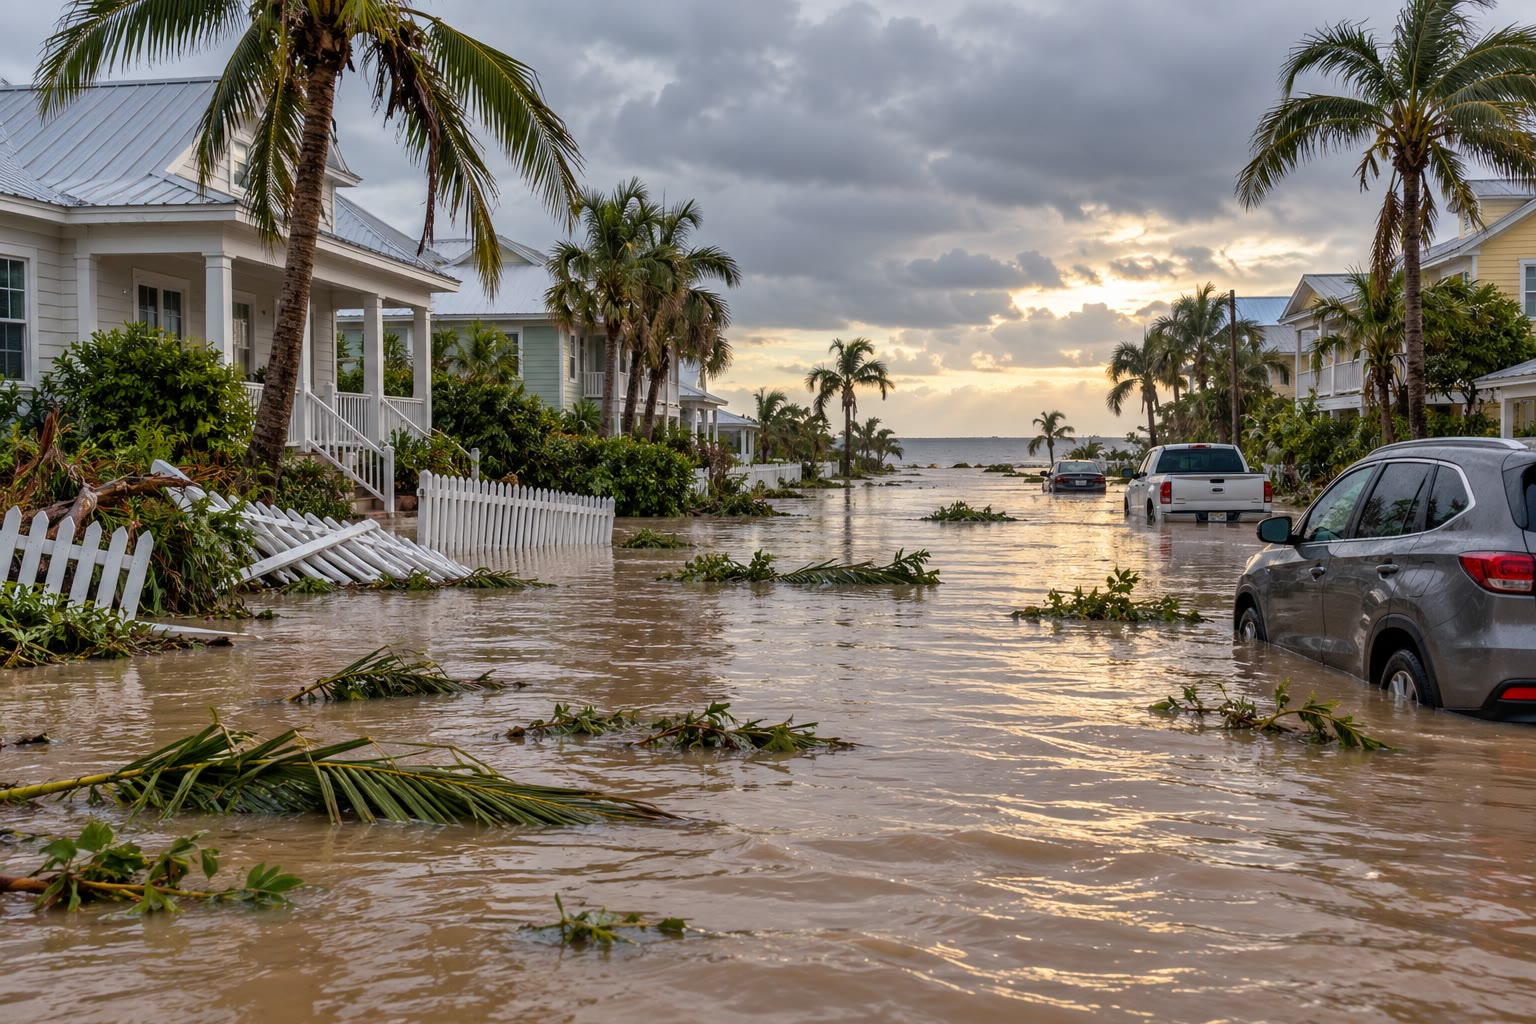
\includegraphics[width=0.7\linewidth]{images/book2/ai/g10-flooded-street.jpg}

{\small Uma rua do litoral na manhã seguinte a uma \omterm{def:g10:storms-and-cyclones:storm-surge}{maré de tempestade}: água
do mar, palmeiras quebradas e cercas arrancadas.}
\end{omfigure}

\section{Exercícios}

\begin{exercise}[$\star$]\label{exo:g10:storms-and-cyclones:1}
Defina uma \omterm{def:g10:storms-and-cyclones:thunderstorm}{trovoada} e o \omterm{def:g10:storms-and-cyclones:lightning}{raio}. O que produz o som do trovão?
\end{exercise}

\begin{exercise}[$\star$]\label{exo:g10:storms-and-cyclones:2}
Defina um \omterm{def:g10:storms-and-cyclones:tropical-cyclone}{ciclone tropical}, o seu \omterm{def:g10:storms-and-cyclones:tropical-cyclone}{olho} e a \omterm{def:g10:storms-and-cyclones:tropical-cyclone}{parede do olho}. Onde os seus
ventos são mais fortes?
\end{exercise}

\begin{exercise}[$\star$]\label{exo:g10:storms-and-cyclones:3}
Em que categoria de Saffir--Simpson fica um furacão com ventos sustentados
de \num{70}~nós? E de \num{120}~nós? E de \num{140}~nós? Quais deles são
furacões intensos?
\end{exercise}

\begin{exercise}[$\star$]\label{exo:g10:storms-and-cyclones:4}
Você conta \num{9} segundos entre um clarão e o seu trovão, e depois
\num{15} segundos para o clarão seguinte. A que distância estava cada um, e
a tempestade está se aproximando?
\end{exercise}

\begin{exercise}[$\star$]\label{exo:g10:storms-and-cyclones:5}
Explique por que uma árvore sozinha num campo é um abrigo perigoso durante
uma \omterm{def:g10:storms-and-cyclones:thunderstorm}{trovoada}, e para onde se deve ir em vez disso.
\end{exercise}

\begin{exercise}[$\star\star$]\label{exo:g10:storms-and-cyclones:6}
Um nó equivale a \qty{1852}{m} por hora. Converta \num{64}~nós e
\num{137}~nós em \unit{m/s} e em \unit{km/h}.
\end{exercise}

\begin{exercise}[$\star\star$]\label{exo:g10:storms-and-cyclones:7}
Há 44 \omterm{def:g10:storms-and-cyclones:lightning}{raios} por segundo na Terra. Quantos são num dia, e num ano?
\end{exercise}

\begin{exercise}[$\star\star$]\label{exo:g10:storms-and-cyclones:8}
Um furacão tem uma pressão central de \qty{935}{hPa} em arredores a
\qty{1010}{hPa}. Qual é a altura da elevação barométrica do mar sob ele?
\end{exercise}

\begin{exercise}[$\star\star$]\label{exo:g10:storms-and-cyclones:9}
Usando o mapa das trajetórias, descreva onde os \omterm{def:g10:storms-and-cyclones:tropical-cyclone}{ciclones tropicais} se formam
e para onde eles vão depois de se formar. Por que eles estão ausentes do
próprio equador?
\end{exercise}

\begin{exercise}[$\star\star$]\label{exo:g10:storms-and-cyclones:10}
A reta do gráfico pressão--vento é $p \approx 1031 - 1.56\,v$ ($p$ em
\unit{hPa}, $v$ em \unit{m/s}). Que pressão central ela dá para o limite
inferior da categoria 5, \qty{70}{m/s}? E para uma tempestade de
\qty{40}{m/s}?
\end{exercise}

\begin{exercise}[$\star\star$]\label{exo:g10:storms-and-cyclones:11}
Explique por que um \omterm{def:g10:storms-and-cyclones:tropical-cyclone}{ciclone tropical} se enfraquece depressa quando passa
sobre a terra, e por que ele se enfraquece sobre águas frias.
\end{exercise}

\begin{exercise}[$\star\star\star$]\label{exo:g10:storms-and-cyclones:12}
A velocidade do som no ar é $\sqrt{1.4\,R\,T/M}$, com $R =
\qty{8.314}{J.mol^{-1}.K^{-1}}$, $T$ em kelvins e $M =
\qty{0.02897}{kg/mol}$. Calcule-a a \qty{0}{\degreeCelsius} e a
\qty{30}{\degreeCelsius}. Para um atraso de \qty{9}{s}, quanto as duas
distâncias diferem? A regra ``\qty{3}{s} por quilômetro'' é boa o bastante?
\end{exercise}

\begin{exercise}[$\star\star\star$]\label{exo:g10:storms-and-cyclones:13}
Uma \omterm{def:g10:storms-and-cyclones:storm-surge}{maré de tempestade} de \qty{4.0}{m} é medida numa costa quando um furacão
com pressão central de \qty{940}{hPa} (arredores a \qty{1010}{hPa}) chega à
terra. Quanto da \omterm{def:g10:storms-and-cyclones:storm-surge}{maré de tempestade} se deve à elevação barométrica, e quanto
ao vento? Se ela chegar na maré alta, \qty{1.5}{m} acima do nível médio do
mar, a que altura acima do nível médio do mar a água chega?
\end{exercise}

\begin{exercise}[$\star\star\star$]\label{exo:g10:storms-and-cyclones:14}
Um \omterm{def:g10:storms-and-cyclones:tornado}{tornado} gira com ventos de \qty{90}{m/s} a \qty{100}{m} do seu eixo; um
furacão, com ventos de \qty{60}{m/s} numa \omterm{def:g10:storms-and-cyclones:tropical-cyclone}{parede do olho} a \qty{30}{km} do
centro. Quanto tempo o ar leva para dar uma volta em cada caso? Compare.
\end{exercise}

\begin{exercise}[$\star\star\star$]\label{exo:g10:storms-and-cyclones:15}
Dos 3\,888 \omterm{def:g10:storms-and-cyclones:tropical-cyclone}{ciclones tropicais} de 1980--2024, 24 atingiram a força de
tempestade tropical a menos de \qty{5}{\degree} do equador, 414 a menos de
\qty{10}{\degree} e 121 além de \qty{30}{\degree}. Calcule as três
porcentagens. A faixa a menos de \qty{5}{\degree} do equador cobre cerca de
\qty{9}{\percent} da superfície da Terra: o que você esperaria se a latitude
não importasse, e o que você conclui?
\end{exercise}

\section{Problema: o motor térmico de um furacão}

\begin{problem}[{Problema de fim de semana --- da chuva de um dia à potência
do vento}]
\label{pb:g10:storms-and-cyclones:1}
% ledger: aoml:energy, nist:water-latent, earth:Rmean, ipcc:budget-toa (all results computed in figdata/grade-10/cyclones.py or from the rounded data below)
Um furacão médio despeja \qty{1.5}{cm} de chuva por dia sobre um círculo de
raio \qty{665}{km}. Use um \omterm{def:g10:earth-energy-budget:latent-heat}{calor latente} de \qty{2.5}{MJ/kg}, uma massa
específica da água de \qty{1000}{kg/m^3}, \qty{86400}{s} num dia e a
potência dos ventos de um furacão médio, \qty{1.5e12}{W}.

\medskip
\noindent\textbf{Parte I --- A chuva de um dia.}
\begin{enumerate}
  \item Calcule a área do círculo.
  \item Calcule o volume de chuva que cai sobre ele num dia.
  \item Expresse-o em quilômetros cúbicos.
  \item Calcule a sua massa.
\end{enumerate}

\medskip
\noindent\textbf{Parte II --- O calor liberado.}
\begin{enumerate}[resume]
  \item Calcule o \omterm{def:g10:earth-energy-budget:latent-heat}{calor latente} liberado num dia pela condensação dessa
        água.
  \item Converta-o numa potência.
  \item A Terra inteira absorve cerca de \qty{1.22e17}{W} de luz solar
        (\cref{ch:g10:earth-energy-budget}). Que fração disso um único
        furacão libera?
  \item A luz solar média absorvida é de \qty{240}{W/m^2}. Calcule a luz
        solar absorvida pela área da tempestade e compare-a com o \omterm{def:g10:earth-energy-budget:latent-heat}{calor
        latente} da tempestade.
  \item O que essa comparação mostra sobre o lugar onde a energia da
        tempestade foi reunida?
\end{enumerate}

\medskip
\noindent\textbf{Parte III --- De onde vem a água.}
\begin{enumerate}[resume]
  \item Que massa de água precisa evaporar a cada dia para alimentar essa
        chuva?
  \item A evaporação média da superfície da Terra leva
        \qty{82}{W/m^2}. Sobre que área a evaporação média forneceria o
        \omterm{def:g10:earth-energy-budget:latent-heat}{calor latente} da tempestade? Compare com a área da tempestade.
  \item Usando a tabela dos teores de saturação do
        \cref{ch:g10:why-clouds-form}, compare a água que um ar saturado
        contém a \qty{28}{\degreeCelsius} e a \qty{20}{\degreeCelsius}.
  \item Explique por que os \omterm{def:g10:storms-and-cyclones:tropical-cyclone}{ciclones tropicais} só se formam sobre mares
        quentes.
  \item Explique por que eles se enfraquecem sobre a terra.
\end{enumerate}

\medskip
\noindent\textbf{Parte IV --- O vento.}
\begin{enumerate}[resume]
  \item Calcule a energia cinética fornecida aos ventos num dia.
  \item Converta o limite inferior da categoria 3, \num{96}~nós, em
        \unit{m/s} (\num{1}~nó = \qty{1852}{m/h}).
  \item O ar perto da superfície do mar tem uma massa específica de cerca
        de \qty{1.16}{kg/m^3}. Calcule a energia cinética de um metro cúbico
        dele movendo-se a essa velocidade.
  \item Compare o \omterm{def:g10:earth-energy-budget:latent-heat}{calor latente} liberado num dia com a energia dos ventos
        num dia.
  \item Em que se transforma o resto do calor liberado?
  \item Que fração do calor liberado pela condensação se torna vento?
\end{enumerate}
\end{problem}
